\section{Table 1: Critical values for Hartley’s $F$ ($F_{max}$)}
\label{table1}

Hartley’s $F_{max}$ tests whether the \concept{assumption} of \concept{homogeneity of variances} is met in your data. This \concept{assumption} entails that the spread (\concept{variance}) of the data should be similar across groups. Hartley’s $F$ is fairly simple to figure out by hand, but it has the requirement that there must be an equal number of observations in each group. \\

Let's consider an example. Suppose that you measured the prices of three brands of soap in $n = 10$ stores. The sample \concept{variances} of the brands $b1$, $b2$, and $b3$, were $s^2_{b1} = 4$, $s^2_{b2} = 7$, and $s^2_{b3} = 10$, respectively. You want to verify the \concept{null hypothesis} that the variances among the brands are equal ($H_0: \sigma^2_{b1} = \sigma^2_{b2} = \sigma^2_{b3}$) against the \concept{alternative hypothesis} that the variances among the brands are unequal ($H_1: \sigma^2_{b1} \neq \sigma^2_{b2} \neq \sigma^2_{b3}$), with 95 percent confidence. \\

Hartley's $F$ is simply the ratio of the largest and the smallest variance: $F = \frac{s^2_{max}}{s^2_{min}}$. In our example, the value of Hartley's $F$ is therefore $\frac{10}{4} = 2.5$. Depending on the number of groups to compare ($k$) and the number of observations ($n$), you can determine the \concept{critical value} of Hartley's $F$ from the table or figure below. \\

If the calculated value is smaller than the critical value, you can retain the \concept{null hypothesis} and conclude that the variances are homogeneous. If the calculated value is larger than the critical value, you must reject the \concept{null hypothesis} and conclude that the variance is not homogeneous. In the example, the calculated value of 2.5 is smaller than the critical value of 6.00, so we can retain the \concept{null hypothesis} that our variance is homogeneous with 95 percent confidence. \\

\begin{raggedright}
\hspace*{0.5cm}
\scriptsize
\begin{tabular}{c|c|c|c|c|c|c|c|c|c|c|c}
\hline
\multicolumn{12}{c}{\textbf{Number of variances to compare} ($k$)}                    \bstrut\tstrut\\
\hline
$n - 1$ & \multicolumn{1}{c}{\textbf{2}}    & \multicolumn{1}{c}{\textbf{3}}    & \multicolumn{1}{c}{\textbf{4}}    & \multicolumn{1}{c}{\textbf{5}}    & \multicolumn{1}{c}{\textbf{6}}    & \multicolumn{1}{c}{\textbf{7}}    & \multicolumn{1}{c}{\textbf{8}}    & \multicolumn{1}{c}{\textbf{9}}    & \multicolumn{1}{c}{\textbf{10}}   & \multicolumn{1}{c}{\textbf{11}}   & \multicolumn{1}{c}{\textbf{12}} \bstrut\tstrut\\
\hline
\textbf{2}     & 39.0 & 87.5 & 142  & 202  & 266  & 333  & 403  & 475  & 550  & 626  & 704  \bstrut\tstrut\\
\textbf{3}     & 15.4 & 27.8 & 39.2 & 50.7 & 62.0 & 72.9 & 83.5 & 93.9 & 104  & 114  & 124  \bstrut\tstrut\\
\textbf{4}     & 9.6  & 15.5 & 20.6 & 25.2 & 29.5 & 33.6 & 37.5 & 41.1 & 44.6 & 48.0 & 51.4 \bstrut\tstrut\\
\textbf{5}     & 7.15 & 10.8 & 13.7 & 16.3 & 18.7 & 20.8 & 22.9 & 24.7 & 26.5 & 28.2 & 29.9 \bstrut\tstrut\\
\textbf{6}     & 5.82 & 8.38 & 10.4 & 12.1 & 13.7 & 15.0 & 16.3 & 17.5 & 18.6 & 19.7 & 20.7 \bstrut\tstrut\\
\textbf{7}     & 4.99 & 6.94 & 8.44 & 9.70 & 10.8 & 11.8 & 12.7 & 13.5 & 14.3 & 15.1 & 15.8 \bstrut\tstrut\\
\textbf{8}     & 4.43 & 6.00 & 7.18 & 8.12 & 9.03 & 9.78 & 10.5 & 11.1 & 11.7 & 12.2 & 12.7 \bstrut\tstrut\\
\textbf{9}     & 4.03 & 5.34 & 6.31 & 7.11 & 7.80 & 8.41 & 8.95 & 9.45 & 9.91 & 10.3 & 10.7 \bstrut\tstrut\\
\textbf{10}    & 3.72 & 4.85 & 5.67 & 6.34 & 6.92 & 7.42 & 7.87 & 8.28 & 8.66 & 9.01 & 9.34 \bstrut\tstrut\\
\textbf{12}    & 3.28 & 4.16 & 4.79 & 5.30 & 5.72 & 6.09 & 6.42 & 6.72 & 7.00 & 7.25 & 7.48 \bstrut\tstrut\\
\textbf{15}    & 2.86 & 3.54 & 4.01 & 4.37 & 4.68 & 4.95 & 5.19 & 5.40 & 5.59 & 5.77 & 5.93 \bstrut\tstrut\\
\textbf{20}    & 2.46 & 2.95 & 3.29 & 3.54 & 3.76 & 3.94 & 4.10 & 4.24 & 4.37 & 4.49 & 4.59 \bstrut\tstrut\\
\textbf{30}    & 2.07 & 2.40 & 2.61 & 2.78 & 2.91 & 3.02 & 3.12 & 3.21 & 3.29 & 3.36 & 3.39 \bstrut\tstrut\\
\textbf{60}    & 1.67 & 1.85 & 1.96 & 2.04 & 2.11 & 2.17 & 2.22 & 2.26 & 2.30 & 2.33 & 2.36 \bstrut\tstrut\\
$\infty$      & 1.00 & 1.00 & 1.00 & 1.00 & 1.00 & 1.00 & 1.00 & 1.00 & 1.00 & 1.00 & 1.00 \bstrut\tstrut\\
\hline
\end{tabular} \\
\hspace*{0.6cm}Level of significance $\alpha = 0.05$
\end{raggedright}

\begin{raggedleft}
\hspace{7cm}
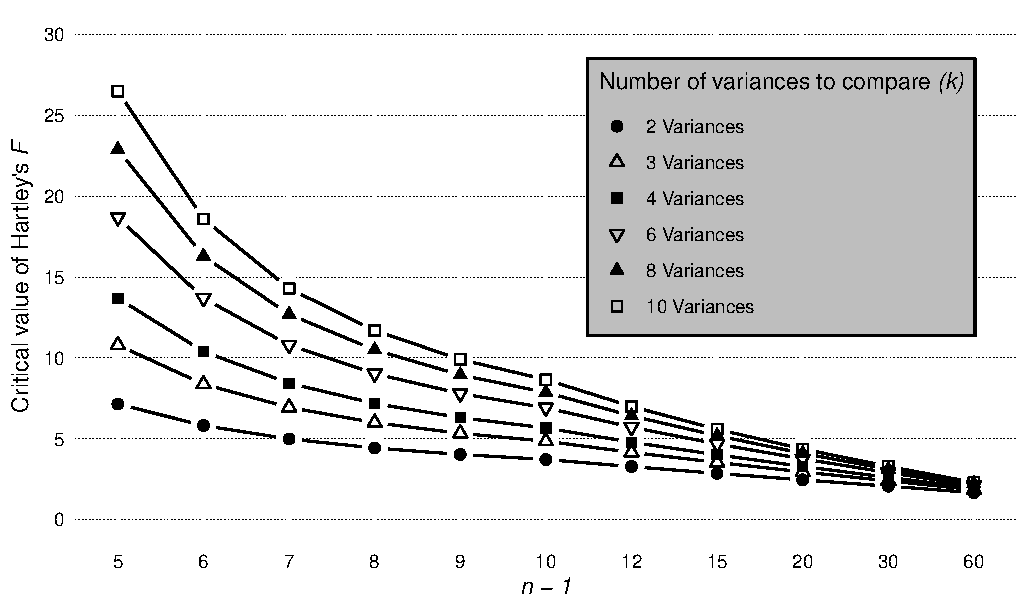
\includegraphics[height = 5.6cm]{Files/Images/HartleysF.pdf}
\end{raggedleft}

\clearpage % Page break